\section{Additional Experiments}\label{sec:additional-results}

In this section we present additional and extended results from the main section.

\subsection{Extended Example of Regularization Paths}%
\label{sec:extended-real-data-paths}

In \Cref{fig:realdata-paths-full} we show an extended example of lasso paths for different
real data sets and types of normalization.

\begin{figure}[hbpt]
  \centering
  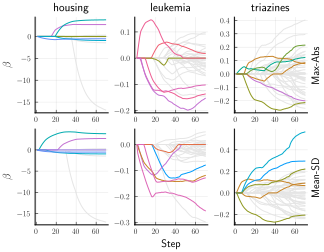
\includegraphics[]{plots/realdata_paths.pdf}
  \caption{%
    Lasso paths for real datasets using two types of normalization:
    standardization and maximum absolute value normalization (max--abs). We have fit
    the lasso path to two different datasets:
    \data{housing}~\citep{harrison1978}, \data{leukemia}~\citep{golub1999},
    \data{triazines}~\citep{king}, and \data{w1a}~\citep{platt1998}. (See \Cref{sec:data-summary}
    for more information about these data sets.) For each
    dataset, we have colored the coefficients if they were among the first five
    to become non-zero under either of the two normalization schemes. We see
    that the paths differ with regards to the size as well as the signs of the
    coefficients, and that, in addition, the features to become active first
    differ between the normalization types.
  }
  \label{fig:realdata-paths-full}
\end{figure}

\subsection{Power and False Discoveries for Multiple Features}%
\label{sec:power-fdr-multiple}

Here, we study how the power of correctly detecting \(k=10\) signals under \(q_j\) linearly
spaced in \([0.5, 0.99]\)~(\Cref{fig:binary-power}). We set \(\beta^*_j = 2\) for each of
the signals, use \(n = 100\,000\), and let \(\sigma_\varepsilon = 1\). The level of
regularization is set to \(\lambda_1 = n 4^\delta/10\). As we can see, the power is
directly related to \(q_j\) and for unbalanced features stronger the higher the choice of
\(\delta\) is.

We also consider a version of the same setup, but with \(p\) linearly spaced in \([20,
    100]\) and compute normalized mean-squared error (NMSE) and false discovery rate
(FDR)~(\Cref{fig:binary-fdr-mse}). As before, we let \(k = 10\) and consider three
different levels of class imbalance. The remaining \(p-k\) features have class balances
spaced evenly on a logarithmic scale from 0.5 to 0.99. Unsurprisingly, the increase in
power gained from selecting \(\delta = 1\) imposes increased false discovery rates. We also
see that the mean-squared error depends on class balance. In line with our previous
results, \(\delta \in \{0, 1/2\}\) appears to work well for balanced features whilst
\(\delta = 1\) works better when there are large imbalances. In the case when \(q_j =
0.99\), the model under scaling with \(\delta = 0\) does not detect any of the true
signals.

\begin{figure*}[htpb]
  \centering
  \subfigure[%
    The power (probability of detecting all true signals) of the lasso. In our orthogonal
    setting, power is constant over \(p\), which is why we have omitted the parameter in the
    plot. \label{fig:binary-power}
  ]{\includegraphics[]{plots/power.pdf}}\hfill%
  \subfigure[%
    NMSE and FDR: the rate of coefficients incorrectly set to non-zero (false discoveries) to
    the total number of estimated coefficients that are nonzero (discoveries).
    \label{fig:binary-fdr-mse}]{\includegraphics[]{plots/fdr_mse.pdf}}%%
  % \includegraphics[]{plots/beta-bias-multidim.pdf}
  \caption{%
    Normalized mean-squared error (NMSE), false discovery rate (FDR), and power for a lasso problem with
    \(k = 10\) true signals (nonzero \(\beta_j^*\)), varying \(p\), and \(q_j \in [0.5, 0.99]\). The noise level is set at \(\sigma_\varepsilon = 1\) and \(\lambda_1 = 0.02\).
  }
\end{figure*}

The results~(\Cref{fig:binary-decreasing}, and \Cref{fig:binary-decreasing-full} in
\Cref{sec:additional-results-biasvar}) show that class balance has considerable effect,
particularly in the case of no scaling (\(\delta = 0\)), which corroborates our theory from
\Cref{sec:theory-binary-features}. At \(q_j=0.99\), for instance, the estimate
(\(\hat{\beta}_{20}\)) is consistently zero when \(\delta = 0\). For \(\delta=1\), we see
that class imbalance increases the variance of the estimates. What is also clear is that
the variance of the estimates increase with class imbalance and that this effect increases
together with \(\delta\).

The level of correlation between the features introduces additional variance in the
estimates but also seems to increase the effect of class imbalance in the cases when
\(\delta = 0\) or \(1/2\).

\begin{figure}[htpb]
  \centering
  \includegraphics[]{plots/binary_decreasing.pdf}
  \caption{%
    Estimates of the regression coefficients from the lasso, \(\hat{\vec{\beta}}\), for the
    first 30 coefficients in the experiment. All of the features are binary and the first 20
    features correspond to true signals with \(\beta_j^* = 2\) and geometrically decreasing
    class balance from 0.5 to 0.99. The remaining features have class balance \(q_j \in [0.5,
      0.99]\) distributed linearly among the features. The plot shows means and standard
    deviations averaged over 50 iterations.
  }
  \label{fig:binary-decreasing-full}
\end{figure}

\subsubsection{Predictive Performance for Simulated Data}%
\label{sec:predictive-performance-simulated}

\begin{figure}[htpb]
  \centering
  \includegraphics[]{plots/hyperopt_surfaces.pdf}
  \caption{%
    Contour plots of normalized mean-squared error (NMSE) for the hold-out validation set
    across a grid of \(\delta\) and \(\lambda\) values for ridge regression and the lasso. The
    dotted path shows the smallest NMSE as a function of \(\lambda\). The dot marks the
    combination with the smallest error.
  }
  \label{fig:hyperopt-contours-full}
\end{figure}

In this experiment, we consider predictive performance in terms of mean-squared error of
the lasso and ridge regression given different levels of class balance (\(q_j \in \{0.5,
0.9, 0.99\}\)), signal-to-noise ratio, and normalization (\(\delta\)). All of the features
are binary, but here we have used \(n=300\) and \(p = \num{1000}\). The \(k=10\) first
features correspond to true signals with \(\beta^*_j = 1\) and all have class balance
\(q\). To set signal-to-noise ratio levels, we rely on the same choice as in
\citet{hastie2020} and use a log-spaced sequence of values from 0.05 to 6. We use standard
hold-out validation with equal splits for training, validation, and test sets. And we fit a
full lasso path, parameterized by a log-spaced grid of 100 values\footnote{This is a
  standard choice of grid, used for instance by \citet{friedman2010}}, from
\(\lambda_\text{max}\) (the value of \(\lambda\) at which the first feature enters the
model) to \(10^{-2}\lambda_\text{max}\) on the training set and pick \(\lambda\) based on
validation set error. Then we compute the hold-out test set error and aggregate the results
across 100 iterations.

The results~(\Cref{fig:binary-sim}) show that the optimal normalization type in terms of
prediction power depends on the class balance of the true signals. If the imbalance is
severe, then we gain by using \(\delta=1/2\) or \(1\), which gives a chance of recovering
the true signals. If everything is balanced, however, then we do better by not scaling. In
general, \(\delta=1/2\) works well for these specific combinations of settings.

\begin{figure}[htpb]
  \centering
  \includegraphics[]{plots/binary_data_sim.pdf}
  \caption{%
    Normalized mean-squared prediction error in a lasso model for different types of
    normalization (\(\delta\)), types of class imbalances (\(q_j\)), and signal-to-noise ratios
    (0.05 to 6) in a data set with \(n=300\) observations and \(p = \num{1000}\) features. The
    error is aggregated test-set error from hold-out validation with \(100\) observations in
    each of the training, validation, and test sets. The plot shows means and Student's
    \(t\)-based 95\% confidence intervals. } \label{fig:binary-sim}
\end{figure}

\

In \Cref{fig:hyperopt-support}, we have, in addition to NMSE on the validation set, also
plotted the size of the support of the lasso (cardinality of the set of features that have
corresponding nonzero coefficients). Here we only show results for \(\delta \in \{0, 1/2,
1\}\). It is clear that \(\delta = 1/2\) works quite well for all of these three data sets,
being able to attain a value close to the mininum for each of the three data sets. This is
not the case for \(\delta \in \{0, 1\}\), for which the best possible prediction error is
considerably worse. This is particularly the case with \(\delta =0\) and the \data{w1a}
data set. The dependency between \(\lambda\) and \(\delta\) is also visible here by looking
at the support size.

\begin{figure}[htpb]
  \centering
  \includegraphics[]{plots/hyperopt_paths.pdf}
  \caption{%
    Support size and normalized mean-squared error (NMSE) for the validation set for the lasso
    fit to datasets \data{a1a}, \data{w1a}, and \data{rhee2006} across combinations of
    \(\delta\) and \(\lambda\). The optimal \(\delta\) is marked with dashed black lines and
    the best combination of \(\delta\) (among 0, 1/2, and 1) and \(\lambda\) is shown as a dot.
  }
  \label{fig:hyperopt-support}
\end{figure}

\subsection{Interactions}%
\label{sec:additional-experiments-interactions}

In \Cref{fig:interactions-full} we show an version of the result in \Cref{fig:interactions}
with different types of signals. Irrespective of the signal, strategy 2 still performs
best.

\begin{figure}[htpb]
  \centering
  \includegraphics[]{plots/interactions-classbalance.pdf}
  \caption{%
    Lasso estimates for a three-feature problem where the third feature is an
    interaction term between the first two features. The first feature is
    binary with class balance \(q\) and the second is quasi-normal with
    standard deviation 0.5. The signal-to-noise ratio is 1. The experiment was
    run for 50 iterations and we aggregate and report means across all
    iterations. Please see \Cref{sec:experiments-interactions} for information
    about the different strategies.
  }
  \label{fig:interactions-full}
\end{figure}

\subsection{The Weighted Elastic Net}%
\label{sec:additional-experiments-weighted-elnet}

In \Cref{fig:mixed-data-elnet-full}, we show a version of \Cref{fig:mixed-data-elnet} with
various settings for \(\alpha\) (the balance between the lasso and ridge penalties). Our
previous conclusions do not seem to be affected by this choice, but as expected the class
balance bias decreases as \(\alpha\) approaches 0 (ridge regression).

\begin{figure}[htpb]
  \centering
  \includegraphics{plots/mixed_data_elnet.pdf}
  \caption{%
    Weighted elastic net estimates for a two-dimensional problem where one feature is a binary
    feature with class balance \(q\) (\(\bernoulli(q)\)), and the other is a quasi-normal
    feature with standard deviation 1/2 (\(\normal(0, 0.5)\)). Here, we have \(n = \num{1000}\)
    observations. The signal-to-noise ratio is 0.5. In every case, we standardize the normal
    feature. The binary feature, meanwhile, is centered by its mean and scaled by
    \((q-q^2)^\delta\). The experiment was run for 50 iterations and we aggregate and report
    means and standard deviations of the estimates.
  }
  \label{fig:mixed-data-elnet-full}
\end{figure}
